% Created by tikzDevice version 0.10.1 on 2017-12-07 15:03:06
% !TEX encoding = UTF-8 Unicode
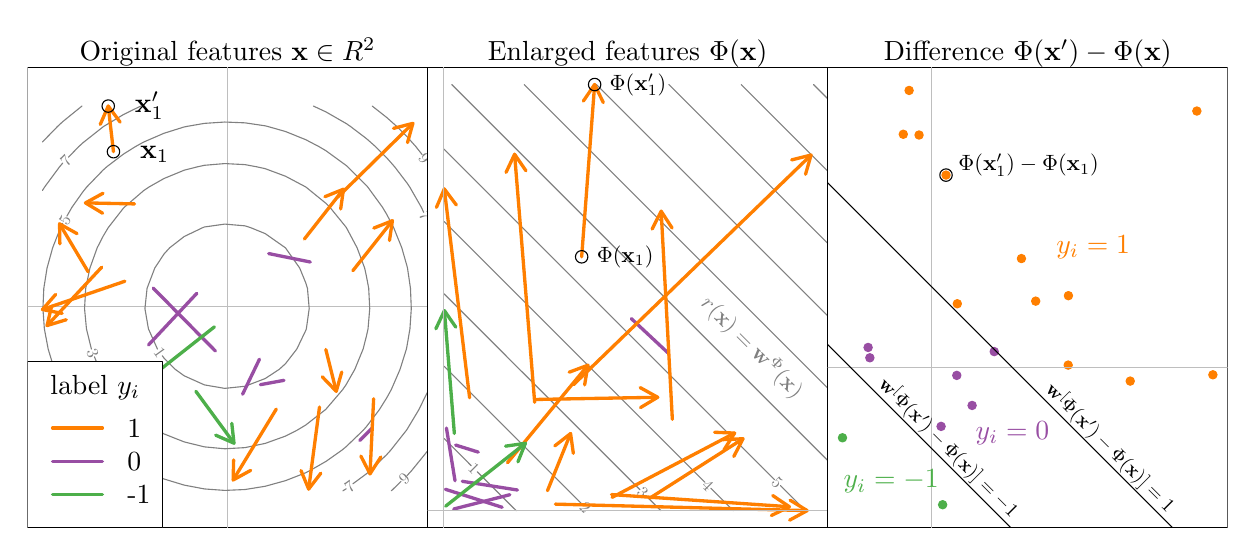
\begin{tikzpicture}[x=1pt,y=1pt]
\definecolor{fillColor}{RGB}{255,255,255}
\path[use as bounding box,fill=fillColor,fill opacity=0.00] (0,0) rectangle (433.62,180.67);
\begin{scope}
\path[clip] (  0.00,  0.00) rectangle (433.62,180.67);
\definecolor{drawColor}{RGB}{0,0,0}

\path[draw=drawColor,line width= 0.4pt,line join=round,line cap=round] (  0.00,  0.00) --
	(144.54,  0.00) --
	(144.54,166.27) --
	(  0.00,166.27) --
	(  0.00,  0.00);
\end{scope}
\begin{scope}
\path[clip] (  0.00,  0.00) rectangle (144.54,166.27);
\definecolor{drawColor}{RGB}{190,190,190}

\path[draw=drawColor,line width= 0.4pt,line join=round,line cap=round] (  0.00, 80.05) -- (144.54, 80.05);

\path[draw=drawColor,line width= 0.4pt,line join=round,line cap=round] ( 72.09,  0.00) -- ( 72.09,166.27);
\end{scope}
\begin{scope}
\path[clip] (  0.00,  0.00) rectangle (433.62,180.67);
\definecolor{drawColor}{RGB}{0,0,0}

\node[text=drawColor,anchor=base,inner sep=0pt, outer sep=0pt, scale=  1.00] at ( 72.27,168.67) {Original features $\mathbf x\in\mathbb R^2$};
\end{scope}
\begin{scope}
\path[clip] (  0.00,  0.00) rectangle (144.54,166.27);
\definecolor{drawColor}{gray}{0.50}

\path[draw=drawColor,line width= 0.4pt,line join=round,line cap=round] ( 46.90, 64.53) --
	( 43.63, 71.85) --
	( 42.37, 79.16) --
	( 43.14, 86.48) --
	( 45.93, 93.80) --
	( 49.26, 98.87) --
	( 51.30,101.12) --
	( 56.57,105.21) --
	( 63.30,108.43) --
	( 63.89,108.65) --
	( 71.21,109.69) --
	( 78.53,109.06) --
	( 80.50,108.43) --
	( 85.84,106.25) --
	( 93.14,101.12) --
	( 93.16,101.10) --
	( 98.30, 93.80) --
	(100.48, 88.46) --
	(101.10, 86.48) --
	(101.73, 79.16) --
	(100.70, 71.85) --
	(100.48, 71.25) --
	( 97.25, 64.53) --
	( 93.16, 59.25) --
	( 90.91, 57.21) --
	( 85.84, 53.88) --
	( 78.53, 51.09) --
	( 71.21, 50.33) --
	( 63.89, 51.58) --
	( 56.57, 54.86) --
	( 53.32, 57.21) --
	( 49.26, 61.27);

\path[draw=drawColor,line width= 0.4pt,line join=round,line cap=round] ( 49.26, 61.27) -- ( 48.66, 62.10);

\node[text=drawColor,rotate=-54.13,anchor=base west,inner sep=0pt, outer sep=0pt, scale=  0.60] at ( 45.23, 63.32) { 1 };

\path[draw=drawColor,line width= 0.4pt,line join=round,line cap=round] ( 27.31, 54.68) --
	( 25.92, 57.21);

\path[draw=drawColor,line width= 0.4pt,line join=round,line cap=round] ( 23.03, 64.53) --
	( 21.24, 71.85) --
	( 20.55, 79.16) --
	( 20.97, 86.48) --
	( 22.49, 93.80) --
	( 25.12,101.12) --
	( 27.31,105.39) --
	( 29.13,108.43) --
	( 34.62,115.48) --
	( 34.88,115.75) --
	( 41.94,121.81) --
	( 43.80,123.07) --
	( 49.26,126.16) --
	( 56.57,129.17) --
	( 61.36,130.39) --
	( 63.89,130.94) --
	( 71.21,131.56) --
	( 78.53,131.18) --
	( 82.78,130.39) --
	( 85.84,129.72) --
	( 93.16,126.99) --
	(100.48,123.12) --
	(100.55,123.07) --
	(107.80,117.17) --
	(109.22,115.75) --
	(115.11,108.51) --
	(115.16,108.43) --
	(119.04,101.12) --
	(121.77, 93.80) --
	(122.43, 90.74) --
	(123.23, 86.48) --
	(123.60, 79.16) --
	(122.99, 71.85) --
	(122.43, 69.31) --
	(121.21, 64.53) --
	(118.21, 57.21) --
	(115.11, 51.76) --
	(113.86, 49.90) --
	(107.80, 42.84) --
	(107.52, 42.58) --
	(100.48, 37.09) --
	( 97.44, 35.26) --
	( 93.16, 33.08) --
	( 85.84, 30.45) --
	( 78.53, 28.92) --
	( 71.21, 28.50) --
	( 63.89, 29.19) --
	( 56.57, 30.98) --
	( 49.26, 33.88) --
	( 46.73, 35.26) --
	( 41.94, 38.35) --
	( 36.79, 42.58) --
	( 34.62, 44.75) --
	( 30.39, 49.90) --
	( 27.31, 54.68);

\path[draw=drawColor,line width= 0.4pt,line join=round,line cap=round] ( 25.92, 57.21) -- ( 24.13, 61.74);

\node[text=drawColor,rotate=-68.44,anchor=base west,inner sep=0pt, outer sep=0pt, scale=  0.60] at ( 21.10, 63.77) { 3 };

\path[draw=drawColor,line width= 0.4pt,line join=round,line cap=round] ( 12.67, 49.98) --
	(  9.63, 57.21) --
	(  7.41, 64.53) --
	(  6.03, 71.85) --
	(  5.51, 79.16) --
	(  5.83, 86.48) --
	(  7.00, 93.80) --
	(  9.02,101.12) --
	( 11.89,108.43) --
	( 12.67,109.97);

\path[draw=drawColor,line width= 0.4pt,line join=round,line cap=round] ( 15.99,115.75) --
	( 19.99,121.41) --
	( 21.33,123.07) --
	( 27.31,129.27) --
	( 28.57,130.39) --
	( 34.62,134.99) --
	( 38.95,137.70) --
	( 41.94,139.35) --
	( 49.26,142.51) --
	( 56.57,144.80) --
	( 57.71,145.02) --
	( 63.89,146.09) --
	( 71.21,146.57) --
	( 78.53,146.28) --
	( 85.84,145.20) --
	( 86.56,145.02) --
	( 93.16,143.15) --
	(100.48,140.19) --
	(105.24,137.70) --
	(107.80,136.19) --
	(115.11,130.86) --
	(115.66,130.39) --
	(122.43,123.61) --
	(122.90,123.07) --
	(128.23,115.75) --
	(129.75,113.20) --
	(132.24,108.43) --
	(135.19,101.12) --
	(137.07, 94.51) --
	(137.25, 93.80) --
	(138.32, 86.48) --
	(138.62, 79.16) --
	(138.13, 71.85) --
	(137.07, 65.66) --
	(136.85, 64.53) --
	(134.56, 57.21) --
	(131.40, 49.90) --
	(129.75, 46.91) --
	(127.04, 42.58) --
	(122.43, 36.53) --
	(121.31, 35.26) --
	(115.11, 29.29) --
	(113.46, 27.94) --
	(107.80, 23.95) --
	(102.02, 20.63) --
	(100.48, 19.84) --
	( 93.16, 16.98) --
	( 85.84, 14.96) --
	( 78.53, 13.78) --
	( 71.21, 13.46) --
	( 63.89, 13.99) --
	( 56.57, 15.37) --
	( 49.26, 17.59) --
	( 42.03, 20.63) --
	( 41.94, 20.67) --
	( 34.62, 25.10) --
	( 30.77, 27.94) --
	( 27.31, 30.89) --
	( 22.93, 35.26) --
	( 19.99, 38.73) --
	( 17.15, 42.58) --
	( 12.71, 49.90) --
	( 12.67, 49.98);

\path[draw=drawColor,line width= 0.4pt,line join=round,line cap=round] ( 14.17,112.57) -- ( 15.99,115.75);

\node[text=drawColor,rotate= 60.15,anchor=base west,inner sep=0pt, outer sep=0pt, scale=  0.60] at ( 14.46,108.95) { 5 };

\path[draw=drawColor,line width= 0.4pt,line join=round,line cap=round] ( 27.31, 15.29) --
	( 20.36, 20.63) --
	( 19.99, 20.95) --
	( 13.00, 27.94) --
	( 12.67, 28.32) --
	(  7.34, 35.26) --
	(  5.35, 38.30);

\path[draw=drawColor,line width= 0.4pt,line join=round,line cap=round] ( 27.84, 14.95) -- ( 27.31, 15.29);

\node[text=drawColor,rotate=-33.12,anchor=base west,inner sep=0pt, outer sep=0pt, scale=  0.60] at ( 26.71, 13.22) { 7 };

\path[draw=drawColor,line width= 0.4pt,line join=round,line cap=round] (  5.35,121.86) --
	(  6.11,123.07) --
	( 11.52,130.39) --
	( 12.67,131.73);

\path[draw=drawColor,line width= 0.4pt,line join=round,line cap=round] ( 18.46,137.70) --
	( 19.99,139.09) --
	( 27.31,144.88) --
	( 27.52,145.02) --
	( 34.62,149.28) --
	( 40.84,152.34);

\path[draw=drawColor,line width= 0.4pt,line join=round,line cap=round] ( 14.76,133.88) -- ( 18.46,137.70);

\node[text=drawColor,rotate= 45.95,anchor=base west,inner sep=0pt, outer sep=0pt, scale=  0.60] at ( 14.16,130.29) { 7 };

\path[draw=drawColor,line width= 0.4pt,line join=round,line cap=round] (142.26,115.75) --
	(138.07,123.07) --
	(137.07,124.54) --
	(132.61,130.39) --
	(129.75,133.64) --
	(125.69,137.70) --
	(122.43,140.57) --
	(116.58,145.02) --
	(115.11,146.02) --
	(107.80,150.22) --
	(103.25,152.34);

\path[draw=drawColor,line width= 0.4pt,line join=round,line cap=round] (143.11,113.93) -- (142.26,115.75);

\node[text=drawColor,rotate=-65.00,anchor=base west,inner sep=0pt, outer sep=0pt, scale=  0.60] at (141.24,113.05) { 7 };

\path[draw=drawColor,line width= 0.4pt,line join=round,line cap=round] (113.90, 13.31) --
	(115.11, 14.06);

\path[draw=drawColor,line width= 0.4pt,line join=round,line cap=round] (122.43, 19.48) --
	(123.77, 20.63) --
	(129.75, 26.41) --
	(131.14, 27.94) --
	(136.92, 35.26) --
	(137.07, 35.48) --
	(141.32, 42.58) --
	(144.38, 48.79);

\path[draw=drawColor,line width= 0.4pt,line join=round,line cap=round] (117.52, 15.85) -- (122.43, 19.48);

\node[text=drawColor,rotate= 36.52,anchor=base west,inner sep=0pt, outer sep=0pt, scale=  0.60] at (116.34, 12.40) { 7 };

\path[draw=drawColor,line width= 0.4pt,line join=round,line cap=round] ( 12.68, 13.31) --
	( 12.67, 13.32) --
	(  5.36, 20.63) --
	(  5.35, 20.64);

\path[draw=drawColor,line width= 0.4pt,line join=round,line cap=round] (  5.35,139.38) --
	( 10.84,145.02) --
	( 12.67,146.71) --
	( 19.60,152.34);

\path[draw=drawColor,line width= 0.4pt,line join=round,line cap=round] (140.26,137.70) --
	(137.07,141.28) --
	(133.32,145.02) --
	(129.75,148.21) --
	(124.50,152.34);

\path[draw=drawColor,line width= 0.4pt,line join=round,line cap=round] (142.53,134.82) -- (140.26,137.70);

\node[text=drawColor,rotate=-51.83,anchor=base west,inner sep=0pt, outer sep=0pt, scale=  0.60] at (140.90,133.54) { 9 };

\path[draw=drawColor,line width= 0.4pt,line join=round,line cap=round] (137.07, 18.79) --
	(138.75, 20.63) --
	(144.38, 27.56);

\path[draw=drawColor,line width= 0.4pt,line join=round,line cap=round] (131.42, 13.31) -- (134.91, 16.70);

\node[text=drawColor,rotate= 44.21,anchor=base west,inner sep=0pt, outer sep=0pt, scale=  0.60] at (136.36, 15.22) { 9 };
\definecolor{drawColor}{RGB}{152,78,163}

\path[draw=drawColor,line width= 1.2pt,line join=round,line cap=round] ( 61.12, 84.67) -- ( 43.66, 66.03);

\path[draw=drawColor,line width= 1.2pt,line join=round,line cap=round] ( 84.09, 51.67) -- ( 92.61, 53.23);

\path[draw=drawColor,line width= 1.2pt,line join=round,line cap=round] (120.03, 31.52) -- (124.47, 36.01);

\path[draw=drawColor,line width= 1.2pt,line join=round,line cap=round] (102.12, 95.99) -- ( 87.09, 99.04);

\path[draw=drawColor,line width= 1.2pt,line join=round,line cap=round] ( 45.37, 86.54) -- ( 67.82, 63.84);

\path[draw=drawColor,line width= 1.2pt,line join=round,line cap=round] ( 77.66, 48.21) -- ( 83.75, 60.87);
\definecolor{drawColor}{RGB}{255,127,0}

\path[draw=drawColor,line width= 1.2pt,line join=round,line cap=round] ( 31.00,135.85) -- ( 29.11,152.34);

\path[draw=drawColor,line width= 1.2pt,line join=round,line cap=round] ( 33.41,146.53) --
	( 29.11,152.34) --
	( 26.23,145.71);

\path[draw=drawColor,line width= 1.2pt,line join=round,line cap=round] (105.45, 43.59) -- (101.53, 13.94);

\path[draw=drawColor,line width= 1.2pt,line join=round,line cap=round] ( 98.77, 20.62) --
	(101.53, 13.94) --
	(105.93, 19.67);

\path[draw=drawColor,line width= 1.2pt,line join=round,line cap=round] (111.97,119.37) -- (139.19,146.09);

\path[draw=drawColor,line width= 1.2pt,line join=round,line cap=round] (137.25,139.13) --
	(139.19,146.09) --
	(132.19,144.28);

\path[draw=drawColor,line width= 1.2pt,line join=round,line cap=round] (117.50, 92.85) -- (131.79,110.91);

\path[draw=drawColor,line width= 1.2pt,line join=round,line cap=round] (130.74,103.76) --
	(131.79,110.91) --
	(125.08,108.25);

\path[draw=drawColor,line width= 1.2pt,line join=round,line cap=round] (125.01, 46.57) -- (123.70, 19.45);

\path[draw=drawColor,line width= 1.2pt,line join=round,line cap=round] (120.40, 25.87) --
	(123.70, 19.45) --
	(127.62, 25.52);

\path[draw=drawColor,line width= 1.2pt,line join=round,line cap=round] (107.73, 64.36) -- (111.50, 49.28);

\path[draw=drawColor,line width= 1.2pt,line join=round,line cap=round] (106.47, 54.48) --
	(111.50, 49.28) --
	(113.49, 56.23);

\path[draw=drawColor,line width= 1.2pt,line join=round,line cap=round] (100.01,104.31) -- (114.12,122.29);

\path[draw=drawColor,line width= 1.2pt,line join=round,line cap=round] (113.10,115.14) --
	(114.12,122.29) --
	(107.41,119.60);

\path[draw=drawColor,line width= 1.2pt,line join=round,line cap=round] ( 89.83, 42.83) -- ( 74.25, 17.23);

\path[draw=drawColor,line width= 1.2pt,line join=round,line cap=round] ( 74.42, 24.46) --
	( 74.25, 17.23) --
	( 80.59, 20.70);

\path[draw=drawColor,line width= 1.2pt,line join=round,line cap=round] ( 26.76, 94.12) -- (  7.01, 73.03);

\path[draw=drawColor,line width= 1.2pt,line join=round,line cap=round] (  8.65, 80.07) --
	(  7.01, 73.03) --
	( 13.93, 75.13);

\path[draw=drawColor,line width= 1.2pt,line join=round,line cap=round] ( 35.13, 89.04) -- (  5.35, 78.82);

\path[draw=drawColor,line width= 1.2pt,line join=round,line cap=round] ( 10.10, 84.27) --
	(  5.35, 78.82) --
	( 12.45, 77.43);

\path[draw=drawColor,line width= 1.2pt,line join=round,line cap=round] ( 21.85, 92.46) -- ( 11.53,109.76);

\path[draw=drawColor,line width= 1.2pt,line join=round,line cap=round] ( 17.84,106.24) --
	( 11.53,109.76) --
	( 11.63,102.53);

\path[draw=drawColor,line width= 1.2pt,line join=round,line cap=round] ( 38.60,116.99) -- ( 20.89,117.35);

\path[draw=drawColor,line width= 1.2pt,line join=round,line cap=round] ( 27.23,120.83) --
	( 20.89,117.35) --
	( 27.08,113.61);
\definecolor{drawColor}{RGB}{77,175,74}

\path[draw=drawColor,line width= 1.2pt,line join=round,line cap=round] ( 67.47, 72.55) -- ( 40.49, 51.29);

\path[draw=drawColor,line width= 1.2pt,line join=round,line cap=round] ( 43.17, 58.00) --
	( 40.49, 51.29) --
	( 47.65, 52.33);

\path[draw=drawColor,line width= 1.2pt,line join=round,line cap=round] ( 60.78, 49.27) -- ( 74.55, 30.52);

\path[draw=drawColor,line width= 1.2pt,line join=round,line cap=round] ( 67.94, 33.42) --
	( 74.55, 30.52) --
	( 73.76, 37.70);
\definecolor{drawColor}{RGB}{0,0,0}
\definecolor{fillColor}{RGB}{255,255,255}

\path[draw=drawColor,line width= 0.4pt,line join=round,line cap=round,fill=fillColor] (  0.00, 60.00) rectangle ( 48.83,  0.00);
\definecolor{drawColor}{RGB}{255,127,0}

\path[draw=drawColor,line width= 1.2pt,line join=round,line cap=round] (  9.00, 36.00) -- ( 27.00, 36.00);
\definecolor{drawColor}{RGB}{152,78,163}

\path[draw=drawColor,line width= 1.2pt,line join=round,line cap=round] (  9.00, 24.00) -- ( 27.00, 24.00);
\definecolor{drawColor}{RGB}{77,175,74}

\path[draw=drawColor,line width= 1.2pt,line join=round,line cap=round] (  9.00, 12.00) -- ( 27.00, 12.00);
\definecolor{drawColor}{RGB}{0,0,0}

\node[text=drawColor,anchor=base,inner sep=0pt, outer sep=0pt, scale=  1.00] at ( 24.42, 48.00) {label $y_i$};

\node[text=drawColor,anchor=base west,inner sep=0pt, outer sep=0pt, scale=  1.00] at ( 36.00, 32.56) {1};

\node[text=drawColor,anchor=base west,inner sep=0pt, outer sep=0pt, scale=  1.00] at ( 36.00, 20.56) {0};

\node[text=drawColor,anchor=base west,inner sep=0pt, outer sep=0pt, scale=  1.00] at ( 36.00,  8.56) {-1};

\path[draw=drawColor,line width= 0.4pt,line join=round,line cap=round] ( 31.00,135.85) circle (  2.25);

\path[draw=drawColor,line width= 0.4pt,line join=round,line cap=round] ( 29.11,152.34) circle (  2.25);

\node[text=drawColor,anchor=base,inner sep=0pt, outer sep=0pt, scale=  1.00] at ( 45.89,133.35) {$\mathbf x_{1}$};

\node[text=drawColor,anchor=base,inner sep=0pt, outer sep=0pt, scale=  1.00] at ( 44.00,149.84) {$\mathbf x_{1}'$};
\end{scope}
\begin{scope}
\path[clip] (  0.00,  0.00) rectangle (433.62,180.67);
\definecolor{drawColor}{RGB}{0,0,0}

\path[draw=drawColor,line width= 0.4pt,line join=round,line cap=round] (144.54,  0.00) --
	(289.08,  0.00) --
	(289.08,166.27) --
	(144.54,166.27) --
	(144.54,  0.00);
\end{scope}
\begin{scope}
\path[clip] (  0.00,  0.00) rectangle (433.62,180.67);
\definecolor{drawColor}{RGB}{0,0,0}

\node[text=drawColor,anchor=base,inner sep=0pt, outer sep=0pt, scale=  1.00] at (216.81,168.67) {Enlarged features $\Phi(\mathbf x)$};
\end{scope}
\begin{scope}
\path[clip] (144.54,  0.00) rectangle (289.08,166.27);
\definecolor{drawColor}{gray}{0.50}

\node[text=drawColor,rotate=-45.00,anchor=base,inner sep=0pt, outer sep=0pt, scale=  0.80] at (260.10, 63.52) {$r(\mathbf x)=\mathbf w^\intercal \Phi(\mathbf x)$};

\path[draw=drawColor,line width= 0.4pt,line join=round,line cap=round] (176.51,  6.16) --
	(174.76,  7.90) --
	(168.40, 14.26) --
	(166.66, 16.00);

\path[draw=drawColor,line width= 0.4pt,line join=round,line cap=round] (160.30, 22.36) --
	(158.56, 24.11) --
	(152.20, 30.47) --
	(150.46, 32.21);

\path[draw=drawColor,line width= 0.4pt,line join=round,line cap=round] (166.66, 16.00) -- (162.42, 20.24);

\node[text=drawColor,rotate=-45.02,anchor=base west,inner sep=0pt, outer sep=0pt, scale=  0.60] at (158.84, 20.90) { 1 };

\path[draw=drawColor,line width= 0.4pt,line join=round,line cap=round] (199.07,  9.73) --
	(194.55, 14.26) --
	(190.97, 17.84) --
	(186.44, 22.36) --
	(182.87, 25.94) --
	(178.34, 30.47) --
	(174.76, 34.04) --
	(170.24, 38.57) --
	(166.66, 42.15) --
	(162.13, 46.67) --
	(158.56, 50.25) --
	(154.03, 54.78) --
	(150.46, 58.35);

\path[draw=drawColor,line width= 0.4pt,line join=round,line cap=round] (200.53,  8.28) -- (199.07,  9.73);

\node[text=drawColor,rotate=-45.02,anchor=base west,inner sep=0pt, outer sep=0pt, scale=  0.60] at (199.07,  6.82) { 2 };

\path[draw=drawColor,line width= 0.4pt,line join=round,line cap=round] (228.79,  6.16) --
	(223.38, 11.57);

\path[draw=drawColor,line width= 0.4pt,line join=round,line cap=round] (220.69, 14.26) --
	(215.28, 19.67) --
	(212.59, 22.36) --
	(207.18, 27.77) --
	(204.48, 30.47) --
	(199.07, 35.88) --
	(196.38, 38.57) --
	(190.97, 43.98) --
	(188.28, 46.67) --
	(182.87, 52.08) --
	(180.17, 54.78) --
	(174.76, 60.18) --
	(172.07, 62.88) --
	(166.66, 68.29) --
	(163.97, 70.98) --
	(158.56, 76.39) --
	(155.86, 79.09) --
	(150.46, 84.49);

\path[draw=drawColor,line width= 0.4pt,line join=round,line cap=round] (221.26, 13.69) -- (220.69, 14.26);

\node[text=drawColor,rotate=-45.02,anchor=base west,inner sep=0pt, outer sep=0pt, scale=  0.60] at (219.80, 12.23) { 3 };

\path[draw=drawColor,line width= 0.4pt,line join=round,line cap=round] (254.93,  6.16) --
	(247.69, 13.40) --
	(246.83, 14.26);

\path[draw=drawColor,line width= 0.4pt,line join=round,line cap=round] (239.59, 21.50) --
	(238.73, 22.36) --
	(231.49, 29.61) --
	(230.62, 30.47) --
	(223.38, 37.71) --
	(222.52, 38.57) --
	(215.28, 45.81) --
	(214.42, 46.67) --
	(207.18, 53.91) --
	(206.31, 54.78) --
	(199.07, 62.02) --
	(198.21, 62.88) --
	(190.97, 70.12) --
	(190.11, 70.98) --
	(182.87, 78.22) --
	(182.01, 79.09) --
	(174.76, 86.33) --
	(173.90, 87.19) --
	(166.66, 94.43) --
	(165.80, 95.29) --
	(158.56,102.53) --
	(157.70,103.40) --
	(150.46,110.64);

\path[draw=drawColor,line width= 0.4pt,line join=round,line cap=round] (244.71, 16.38) -- (239.59, 21.50);

\node[text=drawColor,rotate=-45.02,anchor=base west,inner sep=0pt, outer sep=0pt, scale=  0.60] at (243.25, 14.92) { 4 };

\path[draw=drawColor,line width= 0.4pt,line join=round,line cap=round] (281.08,  6.16) --
	(280.10,  7.13) --
	(272.97, 14.26) --
	(272.00, 15.23);

\path[draw=drawColor,line width= 0.4pt,line join=round,line cap=round] (264.87, 22.36) --
	(263.90, 23.33) --
	(256.77, 30.47) --
	(255.80, 31.44) --
	(248.66, 38.57) --
	(247.69, 39.54) --
	(240.56, 46.67) --
	(239.59, 47.64) --
	(232.46, 54.78) --
	(231.49, 55.75) --
	(224.35, 62.88) --
	(223.38, 63.85) --
	(216.25, 70.98) --
	(215.28, 71.95) --
	(208.15, 79.09) --
	(207.18, 80.06) --
	(200.04, 87.19) --
	(199.07, 88.16) --
	(191.94, 95.29) --
	(190.97, 96.26) --
	(183.84,103.40) --
	(182.87,104.37) --
	(175.74,111.50) --
	(174.76,112.47) --
	(167.63,119.60) --
	(166.66,120.57) --
	(159.53,127.70) --
	(158.56,128.67) --
	(151.43,135.81) --
	(150.46,136.78);

\path[draw=drawColor,line width= 0.4pt,line join=round,line cap=round] (269.88, 17.35) -- (264.87, 22.36);

\node[text=drawColor,rotate=-45.02,anchor=base west,inner sep=0pt, outer sep=0pt, scale=  0.60] at (268.42, 15.89) { 5 };

\path[draw=drawColor,line width= 0.4pt,line join=round,line cap=round] (299.11, 14.26) --
	(296.31, 17.06) --
	(291.01, 22.36) --
	(288.21, 25.17) --
	(282.91, 30.47) --
	(280.10, 33.27) --
	(274.80, 38.57) --
	(272.00, 41.37) --
	(266.70, 46.67) --
	(263.90, 49.48) --
	(258.60, 54.78) --
	(255.80, 57.58) --
	(250.50, 62.88) --
	(247.69, 65.68) --
	(242.39, 70.98) --
	(239.59, 73.79) --
	(234.29, 79.09) --
	(231.49, 81.89) --
	(226.19, 87.19) --
	(223.38, 89.99) --
	(218.08, 95.29) --
	(215.28, 98.09) --
	(209.98,103.40) --
	(207.18,106.20) --
	(201.88,111.50) --
	(199.07,114.30) --
	(193.77,119.60) --
	(190.97,122.40) --
	(185.67,127.70) --
	(182.87,130.51) --
	(177.57,135.81) --
	(174.76,138.61) --
	(169.46,143.91) --
	(166.66,146.71) --
	(161.36,152.01) --
	(158.56,154.82) --
	(153.26,160.12);

\path[draw=drawColor,line width= 0.4pt,line join=round,line cap=round] (302.29, 11.08) -- (299.11, 14.26);

\node[text=drawColor,rotate=-45.02,anchor=base west,inner sep=0pt, outer sep=0pt, scale=  0.60] at (300.83,  9.62) { 6 };

\path[draw=drawColor,line width= 0.4pt,line join=round,line cap=round] (300.95, 38.57) --
	(296.31, 43.21) --
	(292.84, 46.67) --
	(288.21, 51.31) --
	(284.74, 54.78) --
	(280.10, 59.41) --
	(276.64, 62.88) --
	(272.00, 67.52) --
	(268.53, 70.98) --
	(263.90, 75.62) --
	(260.43, 79.09) --
	(255.80, 83.72) --
	(252.33, 87.19) --
	(247.69, 91.82) --
	(244.22, 95.29) --
	(239.59, 99.93) --
	(236.12,103.40) --
	(231.49,108.03) --
	(228.02,111.50) --
	(223.38,116.13) --
	(219.92,119.60) --
	(215.28,124.24) --
	(211.81,127.70) --
	(207.18,132.34) --
	(203.71,135.81) --
	(199.07,140.44) --
	(195.61,143.91) --
	(190.97,148.55) --
	(187.50,152.01) --
	(182.87,156.65) --
	(179.40,160.12);

\path[draw=drawColor,line width= 0.4pt,line join=round,line cap=round] (302.29, 37.22) -- (300.95, 38.57);

\node[text=drawColor,rotate=-45.02,anchor=base west,inner sep=0pt, outer sep=0pt, scale=  0.60] at (300.83, 35.76) { 7 };

\path[draw=drawColor,line width= 0.4pt,line join=round,line cap=round] (304.41, 61.24) --
	(302.78, 62.88);

\path[draw=drawColor,line width= 0.4pt,line join=round,line cap=round] (296.31, 69.35) --
	(294.68, 70.98) --
	(288.21, 77.45) --
	(286.57, 79.09) --
	(280.10, 85.55) --
	(278.47, 87.19) --
	(272.00, 93.66) --
	(270.37, 95.29) --
	(263.90,101.76) --
	(262.26,103.40) --
	(255.80,109.86) --
	(254.16,111.50) --
	(247.69,117.97) --
	(246.06,119.60) --
	(239.59,126.07) --
	(237.95,127.70) --
	(231.49,134.17) --
	(229.85,135.81) --
	(223.38,142.28) --
	(221.75,143.91) --
	(215.28,150.38) --
	(213.64,152.01) --
	(207.18,158.48) --
	(205.54,160.12);

\path[draw=drawColor,line width= 0.4pt,line join=round,line cap=round] (300.66, 65.00) -- (296.31, 69.35);

\node[text=drawColor,rotate=-45.02,anchor=base west,inner sep=0pt, outer sep=0pt, scale=  0.60] at (299.20, 63.54) { 8 };

\path[draw=drawColor,line width= 0.4pt,line join=round,line cap=round] (296.51, 95.29) --
	(296.31, 95.49) --
	(288.41,103.40) --
	(288.21,103.59) --
	(280.30,111.50) --
	(280.10,111.70) --
	(272.20,119.60) --
	(272.00,119.80) --
	(264.10,127.70) --
	(263.90,127.90) --
	(255.99,135.81) --
	(255.80,136.00) --
	(247.89,143.91) --
	(247.69,144.11) --
	(239.79,152.01) --
	(239.59,152.21) --
	(231.68,160.12);

\path[draw=drawColor,line width= 0.4pt,line join=round,line cap=round] (302.29, 89.51) -- (296.51, 95.29);

\node[text=drawColor,rotate=-45.02,anchor=base west,inner sep=0pt, outer sep=0pt, scale=  0.60] at (300.83, 88.05) { 9 };

\path[draw=drawColor,line width= 0.4pt,line join=round,line cap=round] (298.34,119.60) --
	(296.31,121.63) --
	(290.24,127.70) --
	(288.21,129.73) --
	(282.13,135.81) --
	(280.10,137.84) --
	(274.03,143.91) --
	(272.00,145.94) --
	(265.93,152.01) --
	(263.90,154.04) --
	(257.83,160.12);

\path[draw=drawColor,line width= 0.4pt,line join=round,line cap=round] (300.17,117.77) -- (298.34,119.60);

\node[text=drawColor,rotate=-45.02,anchor=base west,inner sep=0pt, outer sep=0pt, scale=  0.60] at (298.71,116.31) { 10 };

\path[draw=drawColor,line width= 0.4pt,line join=round,line cap=round] (304.41,139.67) --
	(300.17,143.91);

\path[draw=drawColor,line width= 0.4pt,line join=round,line cap=round] (292.07,152.01) --
	(288.21,155.88) --
	(283.97,160.12);

\path[draw=drawColor,line width= 0.4pt,line join=round,line cap=round] (295.93,148.15) -- (292.07,152.01);

\node[text=drawColor,rotate=-45.02,anchor=base west,inner sep=0pt, outer sep=0pt, scale=  0.60] at (294.47,146.69) { 11 };
\definecolor{drawColor}{RGB}{152,78,163}

\path[draw=drawColor,line width= 1.2pt,line join=round,line cap=round] (153.96,  6.74) -- (174.24, 11.90);

\path[draw=drawColor,line width= 1.2pt,line join=round,line cap=round] (154.66, 29.84) -- (162.82, 27.30);

\path[draw=drawColor,line width= 1.2pt,line join=round,line cap=round] (218.14, 75.52) -- (231.26, 63.26);

\path[draw=drawColor,line width= 1.2pt,line join=round,line cap=round] (176.99, 13.60) -- (157.04, 16.75);

\path[draw=drawColor,line width= 1.2pt,line join=round,line cap=round] (171.46,  7.36) -- (150.95, 13.86);

\path[draw=drawColor,line width= 1.2pt,line join=round,line cap=round] (151.32, 35.99) -- (154.42, 16.95);
\definecolor{drawColor}{RGB}{255,127,0}

\path[draw=drawColor,line width= 1.2pt,line join=round,line cap=round] (200.18, 97.87) -- (204.87,160.12);

\path[draw=drawColor,line width= 1.2pt,line join=round,line cap=round] (208.00,153.60) --
	(204.87,160.12) --
	(200.79,154.15);

\path[draw=drawColor,line width= 1.2pt,line join=round,line cap=round] (183.20, 45.29) -- (175.95,134.91);

\path[draw=drawColor,line width= 1.2pt,line join=round,line cap=round] (180.05,128.97) --
	(175.95,134.91) --
	(172.85,128.38);

\path[draw=drawColor,line width= 1.2pt,line join=round,line cap=round] (197.26, 51.69) -- (283.07,134.64);

\path[draw=drawColor,line width= 1.2pt,line join=round,line cap=round] (281.08,127.69) --
	(283.07,134.64) --
	(276.06,132.89);

\path[draw=drawColor,line width= 1.2pt,line join=round,line cap=round] (211.18, 10.95) -- (255.45, 34.18);

\path[draw=drawColor,line width= 1.2pt,line join=round,line cap=round] (251.59, 28.07) --
	(255.45, 34.18) --
	(248.23, 34.47);

\path[draw=drawColor,line width= 1.2pt,line join=round,line cap=round] (232.95, 39.14) -- (228.91,114.34);

\path[draw=drawColor,line width= 1.2pt,line join=round,line cap=round] (232.85,108.29) --
	(228.91,114.34) --
	(225.64,107.90);

\path[draw=drawColor,line width= 1.2pt,line join=round,line cap=round] (187.83, 13.37) -- (196.17, 34.00);

\path[draw=drawColor,line width= 1.2pt,line join=round,line cap=round] (197.18, 26.85) --
	(196.17, 34.00) --
	(190.48, 29.55);

\path[draw=drawColor,line width= 1.2pt,line join=round,line cap=round] (173.38, 23.46) -- (202.45, 58.70);

\path[draw=drawColor,line width= 1.2pt,line join=round,line cap=round] (201.26, 51.58) --
	(202.45, 58.70) --
	(195.68, 56.18);

\path[draw=drawColor,line width= 1.2pt,line join=round,line cap=round] (159.69, 46.94) -- (150.55,122.39);

\path[draw=drawColor,line width= 1.2pt,line join=round,line cap=round] (154.89,116.61) --
	(150.55,122.39) --
	(147.71,115.74);

\path[draw=drawColor,line width= 1.2pt,line join=round,line cap=round] (210.97, 11.95) -- (275.23,  7.56);

\path[draw=drawColor,line width= 1.2pt,line join=round,line cap=round] (268.74,  4.39) --
	(275.23,  7.56) --
	(269.23, 11.60);

\path[draw=drawColor,line width= 1.2pt,line join=round,line cap=round] (190.68,  8.50) -- (281.67,  6.16);

\path[draw=drawColor,line width= 1.2pt,line join=round,line cap=round] (275.32,  2.71) --
	(281.67,  6.16) --
	(275.51,  9.93);

\path[draw=drawColor,line width= 1.2pt,line join=round,line cap=round] (224.80, 10.65) -- (258.49, 32.13);

\path[draw=drawColor,line width= 1.2pt,line join=round,line cap=round] (255.15, 25.72) --
	(258.49, 32.13) --
	(251.27, 31.81);

\path[draw=drawColor,line width= 1.2pt,line join=round,line cap=round] (183.47, 46.32) -- (227.66, 47.11);

\path[draw=drawColor,line width= 1.2pt,line join=round,line cap=round] (221.46, 43.39) --
	(227.66, 47.11) --
	(221.33, 50.61);
\definecolor{drawColor}{RGB}{77,175,74}

\path[draw=drawColor,line width= 1.2pt,line join=round,line cap=round] (151.04,  7.77) -- (179.84, 30.48);

\path[draw=drawColor,line width= 1.2pt,line join=round,line cap=round] (177.16, 23.77) --
	(179.84, 30.48) --
	(172.68, 29.45);

\path[draw=drawColor,line width= 1.2pt,line join=round,line cap=round] (154.18, 34.04) -- (150.59, 78.40);

\path[draw=drawColor,line width= 1.2pt,line join=round,line cap=round] (154.70, 72.46) --
	(150.59, 78.40) --
	(147.49, 71.87);
\definecolor{drawColor}{RGB}{0,0,0}

\path[draw=drawColor,line width= 0.4pt,line join=round,line cap=round] (200.18, 97.87) circle (  2.25);

\path[draw=drawColor,line width= 0.4pt,line join=round,line cap=round] (204.87,160.12) circle (  2.25);

\node[text=drawColor,anchor=base,inner sep=0pt, outer sep=0pt, scale=  0.80] at (215.87, 95.87) {$\Phi(\mathbf x_{1})$};

\node[text=drawColor,anchor=base,inner sep=0pt, outer sep=0pt, scale=  0.80] at (220.55,158.12) {$\Phi(\mathbf x_{1}')$};
\definecolor{drawColor}{RGB}{190,190,190}

\path[draw=drawColor,line width= 0.4pt,line join=round,line cap=round] (144.54,  6.11) -- (289.08,  6.11);

\path[draw=drawColor,line width= 0.4pt,line join=round,line cap=round] (150.41,  0.00) -- (150.41,166.27);
\end{scope}
\begin{scope}
\path[clip] (289.08,  0.00) rectangle (433.62,166.27);
\definecolor{drawColor}{RGB}{255,127,0}
\definecolor{fillColor}{RGB}{255,127,0}

\path[draw=drawColor,line width= 0.4pt,line join=round,line cap=round,fill=fillColor] (331.84,127.40) circle (  1.50);
\definecolor{drawColor}{RGB}{152,78,163}
\definecolor{fillColor}{RGB}{152,78,163}

\path[draw=drawColor,line width= 0.4pt,line join=round,line cap=round,fill=fillColor] (349.26, 63.62) circle (  1.50);
\definecolor{drawColor}{RGB}{255,127,0}
\definecolor{fillColor}{RGB}{255,127,0}

\path[draw=drawColor,line width= 0.4pt,line join=round,line cap=round,fill=fillColor] (318.51,157.99) circle (  1.50);

\path[draw=drawColor,line width= 0.4pt,line join=round,line cap=round,fill=fillColor] (422.48,150.54) circle (  1.50);
\definecolor{drawColor}{RGB}{152,78,163}
\definecolor{fillColor}{RGB}{152,78,163}

\path[draw=drawColor,line width= 0.4pt,line join=round,line cap=round,fill=fillColor] (335.73, 55.02) circle (  1.50);
\definecolor{drawColor}{RGB}{255,127,0}
\definecolor{fillColor}{RGB}{255,127,0}

\path[draw=drawColor,line width= 0.4pt,line join=round,line cap=round,fill=fillColor] (376.07, 83.82) circle (  1.50);
\definecolor{drawColor}{RGB}{152,78,163}
\definecolor{fillColor}{RGB}{152,78,163}

\path[draw=drawColor,line width= 0.4pt,line join=round,line cap=round,fill=fillColor] (341.27, 44.16) circle (  1.50);
\definecolor{drawColor}{RGB}{255,127,0}
\definecolor{fillColor}{RGB}{255,127,0}

\path[draw=drawColor,line width= 0.4pt,line join=round,line cap=round,fill=fillColor] (322.10,141.88) circle (  1.50);

\path[draw=drawColor,line width= 0.4pt,line join=round,line cap=round,fill=fillColor] (335.92, 80.91) circle (  1.50);

\path[draw=drawColor,line width= 0.4pt,line join=round,line cap=round,fill=fillColor] (359.09, 97.23) circle (  1.50);
\definecolor{drawColor}{RGB}{152,78,163}
\definecolor{fillColor}{RGB}{152,78,163}

\path[draw=drawColor,line width= 0.4pt,line join=round,line cap=round,fill=fillColor] (304.32, 61.38) circle (  1.50);
\definecolor{drawColor}{RGB}{77,175,74}
\definecolor{fillColor}{RGB}{77,175,74}

\path[draw=drawColor,line width= 0.4pt,line join=round,line cap=round,fill=fillColor] (294.43, 32.48) circle (  1.50);
\definecolor{drawColor}{RGB}{152,78,163}
\definecolor{fillColor}{RGB}{152,78,163}

\path[draw=drawColor,line width= 0.4pt,line join=round,line cap=round,fill=fillColor] (303.69, 65.12) circle (  1.50);

\path[draw=drawColor,line width= 0.4pt,line join=round,line cap=round,fill=fillColor] (330.06, 36.59) circle (  1.50);
\definecolor{drawColor}{RGB}{255,127,0}
\definecolor{fillColor}{RGB}{255,127,0}

\path[draw=drawColor,line width= 0.4pt,line join=round,line cap=round,fill=fillColor] (316.40,142.15) circle (  1.50);

\path[draw=drawColor,line width= 0.4pt,line join=round,line cap=round,fill=fillColor] (398.40, 52.96) circle (  1.50);

\path[draw=drawColor,line width= 0.4pt,line join=round,line cap=round,fill=fillColor] (428.27, 55.24) circle (  1.50);

\path[draw=drawColor,line width= 0.4pt,line join=round,line cap=round,fill=fillColor] (364.25, 81.85) circle (  1.50);

\path[draw=drawColor,line width= 0.4pt,line join=round,line cap=round,fill=fillColor] (375.98, 58.74) circle (  1.50);
\definecolor{drawColor}{RGB}{77,175,74}
\definecolor{fillColor}{RGB}{77,175,74}

\path[draw=drawColor,line width= 0.4pt,line join=round,line cap=round,fill=fillColor] (330.62,  8.29) circle (  1.50);
\end{scope}
\begin{scope}
\path[clip] (  0.00,  0.00) rectangle (433.62,180.67);
\definecolor{drawColor}{RGB}{0,0,0}

\path[draw=drawColor,line width= 0.4pt,line join=round,line cap=round] (289.08,  0.00) --
	(433.62,  0.00) --
	(433.62,166.27) --
	(289.08,166.27) --
	(289.08,  0.00);
\end{scope}
\begin{scope}
\path[clip] (  0.00,  0.00) rectangle (433.62,180.67);
\definecolor{drawColor}{RGB}{0,0,0}

\node[text=drawColor,anchor=base,inner sep=0pt, outer sep=0pt, scale=  1.00] at (361.35,168.67) {Difference $\Phi(\mathbf x')-\Phi(\mathbf x)$};
\end{scope}
\begin{scope}
\path[clip] (289.08,  0.00) rectangle (433.62,166.27);
\definecolor{drawColor}{RGB}{190,190,190}

\path[draw=drawColor,line width= 0.4pt,line join=round,line cap=round] (289.08, 57.86) -- (433.62, 57.86);

\path[draw=drawColor,line width= 0.4pt,line join=round,line cap=round] (326.61,  0.00) -- (326.61,166.28);
\definecolor{drawColor}{RGB}{0,0,0}

\path[draw=drawColor,line width= 0.4pt,line join=round,line cap=round] (289.08,124.59) -- (413.67,  0.00);

\path[draw=drawColor,line width= 0.4pt,line join=round,line cap=round] (289.08, 66.18) -- (355.26,  0.00);

\path[draw=drawColor,line width= 0.4pt,line join=round,line cap=round] (331.84,127.40) circle (  2.25);
\definecolor{drawColor}{RGB}{152,78,163}

\node[text=drawColor,anchor=base,inner sep=0pt, outer sep=0pt, scale=  1.00] at (355.81, 31.91) {$y_i=0$};
\definecolor{drawColor}{RGB}{255,127,0}

\node[text=drawColor,anchor=base,inner sep=0pt, outer sep=0pt, scale=  1.00] at (385.02, 99.08) {$y_i=1$};
\definecolor{drawColor}{RGB}{77,175,74}

\node[text=drawColor,anchor=base,inner sep=0pt, outer sep=0pt, scale=  1.00] at (312.00, 14.38) {$y_i=-1$};
\definecolor{drawColor}{RGB}{0,0,0}

\node[text=drawColor,anchor=base,inner sep=0pt, outer sep=0pt, scale=  0.80] at (361.66,128.88) {$\Phi(\mathbf x_{1}')-\Phi(\mathbf x_{1})$};

\node[text=drawColor,rotate=-45.00,anchor=base,inner sep=0pt, outer sep=0pt, scale=  0.70] at (331.21, 27.41) {$\mathbf w^\intercal [ \Phi(\mathbf x') - \Phi(\mathbf x) ] = -1$};

\node[text=drawColor,rotate=-45.00,anchor=base,inner sep=0pt, outer sep=0pt, scale=  0.70] at (389.63, 27.41) {$\mathbf w^\intercal [ \Phi(\mathbf x') - \Phi(\mathbf x) ] = 1$};
\end{scope}
\end{tikzpicture}
